% !TeX root = ../tfg.tex
% !TeX encoding = utf8

\chapter{Homología persistente}

\section{Complejos de Cech y Vietoris-Rips}
\begin{definicion}
	Sea \(X\) un espacio topológico y sea \(\mathcal{U} = \{U_v\}_{v \in V}\) un recubrimiento de \(X\). Llamaremos \textbf{nervio} de \(\mathcal{U}\) al complejo simplicial abstracto con conjunto de vértices \(V\) tal que la familia \(v_0, \dots, v_p\) genera un \(p\)-símplice si, y sólo si, \(U_{v_0} \cap \dots \cap U_{v_p} \neq \emptyset\). Lo notaremos por \(N(\mathcal{U})\).
\end{definicion}

\begin{teorema}[del Nervio]
	Sea \(X\) un espacio topológico y sea \(\mathcal{U} = \{U_v\}_{v \in V}\) un recubrimiento por abiertos numerable de \(X\). Supongamos además que para todo subconjunto no vacío de vértices \(S \subseteq V\) tenemos que \(\bigcap_{s \in S} U_s\) es contráctil o vacío. Entonces \(N(\mathcal{U})\) es homotópicamente equivalente a \(X\).
\end{teorema}
\begin{proof}
	contenidos...
\end{proof}
\begin{definicion}
	Sea \((X,d)\) un espacio métrico y sea \(V\) un subconjunto de puntos de \(X\).Definimos el \textbf{complejo de CEch} \(C(V, \varepsilon)\) como el nervio \(N(\mathcal{B}_\varepsilon)\), donde
	\[
		\mathcal{B}_\varepsilon = \{ B_{\varepsilon}(v) : v \in V \},
	\]
	siendo \(B_{\varepsilon}(v)\) la bola abierta de centro \(x\) y radio \(\varepsilon > 0\).
\end{definicion}

% Tal vez lo de la variedad pseudoriemanniana

\begin{definicion}
	Sea \((X,d)\) un espacio métrico y sea \(V\) un subconjunto de puntos de \(X\). Definimos el \textbf{complejo de Vietoris-Rips} \(VR(V,\varepsilon)\) como el complejo simplicial cuyo conjunto de vértices es \(V\), de forma que \(\{v_0, v_1, \dots v_p\} \subseteq V\) genera un \(p\)-símplice si, y sólo si, \(d(v_i,v_j) \leq \varepsilon\) para todo \(0 \leq i\), \(j \leq p\).
\end{definicion}
\begin{proposicion}
	Sea \((X,d)\) un espacio métrico y sea \(V\) un subconjunto de puntos de \(X\). Entonces
	\[
		C(V, \varepsilon) \subseteq VR(V, 2\varepsilon) \subseteq C(V, 2\varepsilon).
	\]
\end{proposicion}
\begin{proof}
	La primera imnclusión es inmediata pues si un punto \(x\) pertenece a la intersección \(\bigcap_{v \in V} B(v, \varepsilon)\), entonces la distancia para cada par de puntos de \(V\) es, a lo sumo, \(2 \varepsilon\). En consecuencia, cualquier símplice de \(C(V,\varepsilon)\) se encuentra en \(VR(V, 2\varepsilon)\).
	
	Para la segunda inclusión, consideremos ahora un símplice \(\sigma = \{v_0, \dots, v_p\}\) de \(VR(V, 2\varepsilon)\). Por la definición de complejo de Vietoris-Rips, tenemos que \(d(v_i, v_j) \leq 2\varepsilon\) para todo \(i,j \in \{0, \dots, p\}\). Considerando las bolas abiertas de radio \(2\varepsilon\) centradas en \(v_i\) y en \(v_j\), tenemos que su intersección es no vacía, pues \(v_i \in \overline{B}_{2\varepsilon}(v_j)\) y \(v_j \in \overline{B}_{2\varepsilon}(v_i)\). En el supuesto de que los puntos pertenecieran a la frontera de las bolas, la intersección de las bolas abiertas también sería no vacía pues \(\varepsilon > 0\). En consecuencia, tenemos que \(\sigma \in C(V,2\varepsilon)\).
\end{proof}

\section{Módulos de homología persistente}
\begin{definicion}
	Sea \(K\) un complejo simplicial. Una \textbf{filtración} \(\mathcal{F}\) de \(K\) es una familia totalmente ordenada de subcomplejos \(\{K^n\}_{n \in \N}\) tal que \(\emptyset, K \in \mathcal{F}\) y si \(i \leq j\), entonces \(K^i \subseteq K^j\). En particular, llamaremos a dicho orden \textbf{filtro}.
\end{definicion}
A partir de la definición anterior, podemos construir los complejos de cadenas asociados \(C(K^i;R)\) para todo \(i \in \N\). Así mismo, podemos obtener sus respectivos submódulos de ciclos \(Z^i_p\) y bordes \(B^i_p\) para cada cadena \(C_p(K^i;R)\).
\begin{definicion}
	Sea \(\mathcal{F}\) una filtración, sea \(p\) un número natural y sean \(i,j \in \{0, \dots, n\}\). Definimos el  \textbf{\((i,j)\)-ésimo \(R\)-módulo de homología persistente de nivel \(p\)} asociado a \(\mathcal{F}\) como
	\[
		H_p^{i \to j}(\mathcal{F}) := \im f_p^{i,j}.
	\]
	El rango de \(H_p^{i \to j}(\mathcal{F})\) diremos que es el \textbf{\((i,j)\)-ésimo número de Betti de persistencia de nivel \(p\)} y lo notaremos por \(\beta_p^{i,j}\).
\end{definicion}
\begin{proposicion}
	Sea \(\mathcal{F}\) una filtración del complejo simplicial \(K\). Entonces
	\[
		H_p^{i \to j}(\mathcal{F}) \cong \frac{Z_p(K_j)}{B_p(K_j) \cap Z_p(K_i)}
	\]
	es un isomorfismo de \(R\)-módulos.
\end{proposicion}
\begin{proof}
	Sabemos que el cociente anterior está bien definid,o pues \(Z_p(K_i) \cap B_p(K_j)\) es un submódulo de \(Z_p(K_i)\). Para ver que en efecto existe un isomorfismo, consideraremos la proyección canónica \(\pi_i : Z_p(K_i) \to H_p(K_j)\). Aplicando el \nameref{teo:first-iso}, tenemos que 
	\[
		\frac{Z_p(K_i)}{\ker \pi_i} \cong \im \pi_i
	\]
	es un isomorfismo. Sin embargo, nótese que
	\begin{align*}
		\ker \pi_i &= \{z \in Z_p(K_i) : \pi_i(z) = [0] \}
				   = \{z \in Z_p(K_i) : [z] = [0] \} \\ 
				   &= \{z \in Z_p(K_i) : z \in B_p(K_j) \}
				   = B_p(K_j) \cap Z_p(K_i).
	\end{align*}
	Además, 
	\begin{align*}
		H_p^{i,j}(\mathcal{F}) &= \im f_p^{i,j} = \{f_p^{i,j}([z]) : [z] \in H_p(K_i) \} \\ 
							   &= \{[({i_{i,j}}_*)_p(z)] : z \in Z_p(K_i) \}  
							   = \{\pi_i(z) : z \in Z_p(K_i) \} 
							   = \im \pi_i.
	\end{align*}
\end{proof}

\tikzset{every picture/.style={line width=0.75pt}} %set default line width to 0.75pt        

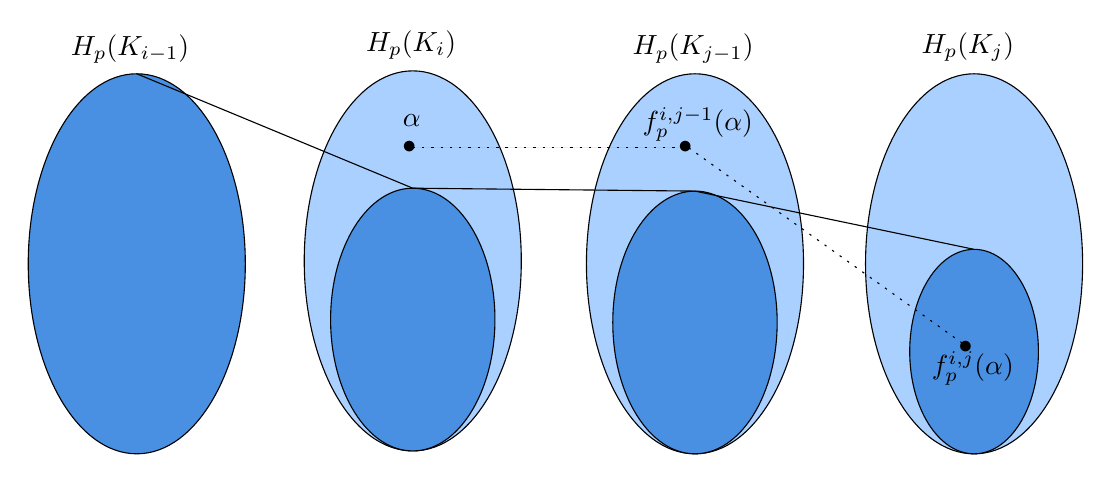
\begin{tikzpicture}[x=0.75pt,y=0.75pt,yscale=-1,xscale=1]
	%uncomment if require: \path (0,235); %set diagram left start at 0, and has height of 235
	
	%Shape: Ellipse [id:dp28793519162441483] 
	\draw  [fill={rgb, 255:red, 74; green, 144; blue, 226 }  ,fill opacity=1 ] (81,72.52) .. controls (81,21.96) and (104.41,-19.03) .. (133.29,-19.03) .. controls (162.18,-19.03) and (185.59,21.96) .. (185.59,72.52) .. controls (185.59,123.08) and (162.18,164.07) .. (133.29,164.07) .. controls (104.41,164.07) and (81,123.08) .. (81,72.52) -- cycle ;
	%Shape: Ellipse [id:dp5681689316325549] 
	\draw  [fill={rgb, 255:red, 169; green, 208; blue, 255 }  ,fill opacity=1 ] (213.98,71.12) .. controls (213.98,20.55) and (237.39,-20.44) .. (266.27,-20.44) .. controls (295.15,-20.44) and (318.56,20.55) .. (318.56,71.12) .. controls (318.56,121.68) and (295.15,162.67) .. (266.27,162.67) .. controls (237.39,162.67) and (213.98,121.68) .. (213.98,71.12) -- cycle ;
	%Shape: Ellipse [id:dp8309047921029127] 
	\draw  [fill={rgb, 255:red, 169; green, 208; blue, 255 }  ,fill opacity=1 ] (349.94,72.52) .. controls (349.94,21.96) and (373.35,-19.03) .. (402.24,-19.03) .. controls (431.12,-19.03) and (454.53,21.96) .. (454.53,72.52) .. controls (454.53,123.08) and (431.12,164.07) .. (402.24,164.07) .. controls (373.35,164.07) and (349.94,123.08) .. (349.94,72.52) -- cycle ;
	%Shape: Ellipse [id:dp6471754723664047] 
	\draw  [fill={rgb, 255:red, 169; green, 208; blue, 255 }  ,fill opacity=1 ] (484.41,72.52) .. controls (484.41,21.96) and (507.82,-19.03) .. (536.71,-19.03) .. controls (565.59,-19.03) and (589,21.96) .. (589,72.52) .. controls (589,123.08) and (565.59,164.07) .. (536.71,164.07) .. controls (507.82,164.07) and (484.41,123.08) .. (484.41,72.52) -- cycle ;
	%Shape: Ellipse [id:dp2887350161913229] 
	\draw  [fill={rgb, 255:red, 74; green, 144; blue, 226 }  ,fill opacity=1 ] (226.68,99.38) .. controls (226.68,64.42) and (244.4,36.09) .. (266.27,36.09) .. controls (288.14,36.09) and (305.86,64.42) .. (305.86,99.38) .. controls (305.86,134.33) and (288.14,162.67) .. (266.27,162.67) .. controls (244.4,162.67) and (226.68,134.33) .. (226.68,99.38) -- cycle ;
	%Shape: Ellipse [id:dp5997979826300346] 
	\draw  [fill={rgb, 255:red, 74; green, 144; blue, 226 }  ,fill opacity=1 ] (362.64,100.78) .. controls (362.64,65.83) and (380.37,37.49) .. (402.24,37.49) .. controls (424.1,37.49) and (441.83,65.83) .. (441.83,100.78) .. controls (441.83,135.73) and (424.1,164.07) .. (402.24,164.07) .. controls (380.37,164.07) and (362.64,135.73) .. (362.64,100.78) -- cycle ;
	%Shape: Ellipse [id:dp7175957985808079] 
	\draw  [fill={rgb, 255:red, 74; green, 144; blue, 226 }  ,fill opacity=1 ] (505.7,114.81) .. controls (505.7,87.61) and (519.58,65.55) .. (536.71,65.55) .. controls (553.83,65.55) and (567.71,87.61) .. (567.71,114.81) .. controls (567.71,142.02) and (553.83,164.07) .. (536.71,164.07) .. controls (519.58,164.07) and (505.7,142.02) .. (505.7,114.81) -- cycle ;
	%Straight Lines [id:da9382562350971808] 
	\draw    (133.29,-19.03) -- (266.27,36.09) ;
	%Straight Lines [id:da8538877694649378] 
	\draw    (266.27,36.09) -- (402.24,37.49) ;
	%Straight Lines [id:da415521229926751] 
	\draw    (402.24,37.49) -- (536.71,65.55) ;
	%Straight Lines [id:da5906511807851325] 
	\draw [fill={rgb, 255:red, 74; green, 144; blue, 226 }  ,fill opacity=1 ] [dash pattern={on 0.84pt off 2.51pt}]  (266.27,16.65) -- (399.25,16.65) ;
	%Straight Lines [id:da7445210416359846] 
	\draw  [dash pattern={on 0.84pt off 2.51pt}]  (399.25,16.65) -- (536.71,114.81) ;
	
	% Text Node
	\draw (260.27,-0.47) node [anchor=north west][inner sep=0.75pt]    {\(\alpha \)};
	% Text Node
	\draw (375.75,-4.04) node [anchor=north west][inner sep=0.75pt]    {\(f_{p}^{i,j-1}( \alpha )\)};
	% Text Node
	\draw (515.12,113.56) node [anchor=north west][inner sep=0.75pt]    {\(f_{p}^{i,j}( \alpha )\)};
	% Text Node
	\draw (100.29,-38.98) node [anchor=north west][inner sep=0.75pt]    {\(H_{p}( K_{i-1})\)};
	% Text Node
	\draw (242.52,-40.98) node [anchor=north west][inner sep=0.75pt]    {\(H_{p}( K_{i})\)};
	% Text Node
	\draw (370.99,-39.38) node [anchor=north west][inner sep=0.75pt]    {\(H_{p}( K_{j-1})\)};
	% Text Node
	\draw (510.2,-39.98) node [anchor=north west][inner sep=0.75pt]    {\(H_{p}( K_{j})\)};
	% Text Node
	\draw (260,12.4) node [anchor=north west][inner sep=0.75pt]    {\(\bullet \)};
	% Text Node
	\draw (393,12.4) node [anchor=north west][inner sep=0.75pt]    {\(\bullet \)};
	% Text Node
	\draw (528,108.4) node [anchor=north west][inner sep=0.75pt]    {\(\bullet \)};
	
	
\end{tikzpicture}

\begin{definicion}
	Dada una filtración \(F\), decimos que un elemento \(\alpha \neq 0\) en \(H^p(K_i)\) nace en \(K_i\) si \(\alpha \not\in H^{p-1}(K_{i-1},F)\). Además, decimos que \(\alpha\) muere entrando en \(K_j\) si se fusiona con una clase proveniente de un nivel anterior cuando se desplaza de \(K_j\) a \(K_{j-1}\); es decir, si \(f_{i,j-1}^p(\alpha) \not\in H^{p-1}(K_{i-1},F)\) pero \(f_{i,j}^p(\alpha) \in H^{p-1}(K_j,F)\).
\end{definicion}

\section{Representación de la homología persistente}
\begin{lema}
	Sea \( A \) un \( R \)-módulo. \( A \) es finitamente generado por \( n \) elementos si, y sólo si, existe un epimorfismo \( \phi : R^n \to A \).
\end{lema}

\begin{proof}
	Sea \( M \) un módulo generado por un conjunto finito de elementos \( \{m_1, \ldots, m_n\} \). Consideremos el homomorfismo \( \phi: R^n \rightarrow M \) definido por
	\[
	\phi(a_1, \ldots, a_n) = \sum_{i=1}^n a_i m_i.
	\]
	Este homomorfismo \( \phi \) es claramente sobreyectivo, ya que cada elemento \( m \) en \( M \) puede ser expresado como \( \phi(a_1, \ldots, a_n) \) para algunos \( a_1, \ldots, a_n \in R \).
	
	Por otro lado, si existe un homomorfismo sobreyectivo \( \phi: R^n \rightarrow M \), entonces, para cada \( m \in M \) existe una \( n \)-tupla \( (a_1, \ldots, a_n) \) en \( R^n \) tal que \( \phi(a_1, \ldots, a_n) = m \). Los elementos \( \phi(e_i) \), donde \( e_i \) es el \( i \)-ésimo vector de la base canónica de \( R^n \), generan \( M \). De aquí se sigue que \( M \) es finitamente generado.
\end{proof}

\begin{definicion}
	Sea \( A \) un \( R \)-módulo finitamente generado por \( n \) elementos y sea \( \phi : R^n \to A \) un epimorfismo. Diremos que \( A \) es \textbf{finitamente presentado} si \( \ker \phi \) es finitamente generado.
\end{definicion}

\begin{definicion}ARREGLAR
	Sea \( \{M_i\}_{i \in \mathbb{N}} \) una familia de \( R \)-módulos. Diremos que dicha familia es un \textbf{módulo de persistencia discreto} sobre el anillo \( R \) si para cada \( i \leq j \) existe un homomorfismo de \( R \)-módulos \( f_{i,j}: A_i \to A_j \) tal que:
	\begin{enumerate}
		\item \( f_{i,i} = \mathrm{id}_{A_i} \) para todo \( i \in \mathbb{N} \).
		\item \( f_{j,k} \circ f_{i,j} = f_{i,k} \) para todo \( i \leq j \leq k \).
	\end{enumerate}
\end{definicion}

\begin{definicion}
	Sean \(\mathcal{M} = \{\{M_i\}_{i \in \N}, \{f_{i,j}\}_{i \leq j \in \N}\}, \mathcal{N} = \{\{N_i\}_{i \in \N}, \{g_{i,j}\}_{i \leq j \in \N}\} \) dos módulos de persistencia discretos.  Diremos que la familia de homomorfismos \(\varphi_\bullet = \{\varphi_i\}_{i \in \N}\) tales que \(\varphi_i : M_i \to N_i\) es un \textbf{homomorfismo de módulos de persistencia discreto} si \(g_{i,j} \circ \varphi_i = \varphi_j \circ f_{i,j}\).
\end{definicion}
La anterior definición es equivalente a decir que el diagrama
\[
	\xymatrix{
		M_0 \ar@{->}[r]^{f_0} \ar@{->}[d]^{\varphi_0} & M_1 \ar@{->}[r]^{f_1} \ar@{->}[d]^{\varphi_1} & \cdots \ar@{->}[r]^{f_{i-1}} & M_i \ar@{->}[r]^{f_i} \ar@{->}[d]^{\varphi_i} & M_{i+1} \ar@{->}[r]^{f_{i+1}} \ar@{->}[d]^{\varphi_{i+1}} & \cdots \\
		N_0 \ar@{->}[r]^{g_0} & N_1 \ar@{->}[r]^{g_1} & \cdots \ar@{->}[r]^{g_{i-1}} & N_i \ar@{->}[r]^{g_i} & N_{i+1} \ar@{->}[r]^{g_{i+1}} & \cdots
	}
\]
conmuta. En las condiciones anteriores, los módulos de persistencia discretos junto a sus homomorfismos forman una categoría que notaremos por \(R\)-\(\Cat{PersMod}\).

\begin{definicion}
	Sea \( R \) un anillo. Diremos que \( R \) es un \textbf{anillo graduado} si puede descomponerse como una suma directa
	\[
	R = \bigoplus_{n=0}^{\infty} R_n,
	\]
	donde \( R_m R_n \subseteq R_{m+n} \) para todos \( m, n \in \mathbb{Z} \). Los elementos de \( R_n \) distintos de cero se denominan \textbf{homogéneos de grado \( n \)}.
\end{definicion}

\begin{definicion}
	Sea \( R \) un anillo graduado y sea \( M \) un \( R \)-módulo. Diremos que \( M \) es un \textbf{módulo graduado} si puede escribirse como
	\[
	M = \bigoplus_{n=0}^{\infty} M_n,
	\]
	donde \( M_n \) son grupos abelianos y \( R_m M_n \subseteq M_{m+n} \) para todos \( m, n \in \mathbb{Z} \). Un elemento de \( M_n \) distinto de cero se llama \textbf{homogéneo de grado \( n \)}.
\end{definicion}

VER QUE LOS MODULOS RGADUADOS FORMAN UNA CATEGORIA

Los módulos de persistencia discretos sobre un anillo \(R\) y los \(R[t]\)-módulos graduados son conceptos íntimamente relacionados. Si \(\mathcal{M}\) es un módulo de persistencia discreto, podemos definir un \(R[t]\)-módulo graduado \(\alpha(\mathcal{M})\) como
\[
	\alpha(\mathcal{M}) = \bigoplus_{i \in \N} M_i,
\]
donde el producto por \(t\) lo definimos como \(t \cdot m_i = f_{i,i+1}(m_i)\) para todo \(m_i \in M_i\). Análogamente, podemos definir un módulo de persistencia discreto a partir de un \(R[t]\)-módulo \(\bigoplus_{i \in \N} M_i\), de forma que
\[
	\beta \left( \bigoplus_{i \in \N} M_i \right) = \mathcal{M}.
\]
Aquí, los morfismos los obtenemos a partir del producto por \(t\), esto es, \(f_{i, i+1}(m_i) = t \cdot m_i\) para todo \(m_i \in M_i\). El siguiente resultado nos proporciona formalmente cómo de íntima 
es esta relación.

\begin{lema}
	Las aplicaciones \(\alpha\) y \(\beta\) definidas anteriormente forman una pareja isomorfa de funtores entre \(R\)-\(\Cat{PersMod}\) y \(R[t]\)-\(\Cat{Gr}\text{-}\Cat{Mod}\). En particular, ambas categorías son isomorfas.
\end{lema}
\begin{proof}
	Sea \(\varphi_\bullet : \mathcal{M} \to \mathcal{N}\) un morfismo de módulos de persistencia discretos. Definamos
	\[
		\alpha(\varphi_{\bullet}) : \bigoplus_{i \in \N} M_i \to \bigoplus_{i \in \N} N_i
	\]
	donde a cada \(m_i \in M_i\) le asignamos \(\varphi_i(m_i)\) para cada \(i \in \N\). Veamos que \(\alpha : R\)-\(\Cat{PersMod} \to R[t]\)-\(\Cat{Gr}\text{-}\Cat{Mod}\) es un funtor. Primero veamos que \(\alpha(\varphi_{\bullet})\) es un morfismo de módulos graduados. Tenemos que \(\alpha(\varphi_{\bullet})\) es un homomorfismo de grupos pues cada \(\varphi_{i}\) lo es, cumple que \(\alpha(\varphi_{i})(M_i) \subseteq N_i\) y además, si \(m = (m_0, m_1, \ldots)\) es un elemento de \(\mathcal{M}\), entonces
	\begin{align*}
		\alpha(\varphi_{\bullet})(tm) &= \alpha(\varphi_{\bullet})(0, tm_0, tm_1, \ldots) = (0, \varphi_0(tm_0), \varphi_1(tm_1), \ldots) \\
		&= (0, t\varphi_0(m_0), t\varphi_1(m_1), \ldots) = t\alpha(\varphi_{\bullet})(m),
	\end{align*}
	donde la última igualdad es consecuencia de la propiedad \((2)\) de los morfismos de módulos de persistencia discretos. 
	En cuanto a las propiedades funtoriales, es evidente que \(\alpha\) lleva identidades en identidades. Además, si \(\psi_\bullet\) es otro morfismo de módulos de peristencia discretos, tenemos que
	\begin{align*}
		(\alpha(\psi_\bullet \circ \varphi_\bullet))(m) = (\psi_i(\varphi_i(m_i)))_{i \in \N} = \alpha (\psi_\bullet)(\varphi_i(m_i))_{i \in \N} = (\alpha(\psi_\bullet) \circ \alpha(\varphi_\bullet))(m).
	\end{align*}
	
	Consideremos ahora el homomorfismo de \(R[t]\)-módulos graduados
	\[
		\eta : \bigoplus_{i \in \N} M_i \to \bigoplus_{i \in \N} N_i,
	\]
	que para cada \(i \in \N\) induce un homomorfismo \(\eta_i : M_i \to N_i\) compatible con el producto por \(t\). En consecuencia, el diagrama
	\[
	\xymatrix{
		M_0 \ar@{->}[r]^{t} \ar@{->}[d]^{\eta_0} & M_1 \ar@{->}[r]^{t} \ar@{->}[d]^{\eta_1} & \cdots \ar@{->}[r]^{t} & M_i \ar@{->}[r]^{t} \ar@{->}[d]^{\eta_i} & M_{i+1} \ar@{->}[r]^{t} \ar@{->}[d]^{\eta_{i+1}} & \cdots \\
		N_0 \ar@{->}[r]^{t} & N_1 \ar@{->}[r]^{t} & \cdots \ar@{->}[r]^{t} & N_i \ar@{->}[r]^{t} & N_{i+1} \ar@{->}[r]^{t} & \cdots
	}
	\]
	es conmutativo. Definamos ahora \(\beta(\eta) = (\eta_0, \eta_1, \ldots)\) y veamos que es un homomorfismo de módulos de persistencia discretos entre \(\mathcal{M}\) y \(\mathcal{N}\). En consecuencia, \(\beta\) nos da homomorfismos de grupos \(\eta_i : M_i \to N_i\) que, a su vez, son homomorfismos de \(R\)-módulos. Para comprobarlo, basta tomar cualquier \(r \in R\) y \(m_i \in M_i\) y vemos que \(\eta_i(rm_i) = \eta(rm_i) = r \eta(m_i) = r \eta_i(m_i)\). Como los homomorfismos de \(R\)-módulos de \(\mathcal{M}\) y \(\mathcal{N}\) se obtienen mediante la multiplicación por \(t\), entonces para todo \(m_i \in M_i\) tenemos que
	\[
		\eta_{i+1}(tm_i) = \eta(tm_i) = t\eta(m_i) = t \eta_i(m_i),
	\]
	por lo que \(\beta(\eta)\) es un homomorfismo de módulos de persistencia discretos.
	Claramente \(\beta\) conserva la identidad. Luego para otro \(\theta : \mathcal{M} \to \mathcal{N}\) y cualquier \(m=(m_i)_{i \in \N} \in \mathcal{M}\),
	\[
		(\beta(\theta \circ \eta))(m) = (\theta(\eta(m_i)))_{i \in \N} = \beta(\theta)(\eta(m_i))_{i \in \N} = (\beta(\theta) \circ \beta(\eta))(m).
	\]
	Esto es, \(\beta\) es un funtor. Finalmente, por la construcción de \(\alpha\) y \(\beta\) tenemos que \(\beta \circ \alpha\) es el funtor identidad en \(R[t]\)-\(\Cat{Gr}\text{-}\Cat{Mod}\) y que \(\alpha \circ \beta\) es el funtor identidad en \(R\)-\(\Cat{PersMod}\).
\end{proof}

En la práctica generalmente trabajaremos con módulos de persistencia que cumplen ciertas condiciones de finitud. Por ello, resulta de gran interés conocer si la correspondencia recién realizada se sigue cumpliendo bajo estos casos.

\begin{definicion}
	Diremos que un módulo de persistencia discreto \(\mathcal{M}\) es de \textbf{tipo finito} si existe \(n \in \N\) de forma que para todo \(i,j \in \N\) tal que \(n \leq i \leq j\) la aplicación \(f_{i,j}\) es un isomorfismo.
\end{definicion}

\begin{definicion}
	Diremos que un módulo de persistencia discreto \(\mathcal{M}\) es de \textbf{finitamente presentado (generado)} si es de tipo finito y además, \(M_i\) es finitamente presentado (generado) para todo \(i \in \N\).
\end{definicion}

\begin{lema}
	Sea \(\mathcal{M}\) un módulo de persistencia discreto. Si \(\mathcal{M}\) es finitamente presentado, entonces \(\alpha(\mathcal{M})\) es finitamente presentado.
\end{lema}
\begin{proof}
	Consideremos \(N \in \N\) de forma que \(f_{i,j} : M_i \to N_i\) es un isomorfismo para todo \(N \leq i \leq j\). Sea \(G\) un conjunto de generadores de \(M_i\). Queremos ver que \(G = \bigcup_{i=1}^N G_i\) es un sistema de generadores también para \(\alpha(\mathcal{M})\). Para ello, veamos que todo elemento homogéneo de \(\alpha(\mathcal{M})\) está generado por la unión de los \(G_i\). Fijemos \(k \in \N\) y sea \(m_k \in \alpha(\mathcal{M})\) un elemento homogéneo de grado \(k\). Si \(k \leq N\), entonces \(m_k\) está generado por los elementos de \(G_k\) por construcción. Si \(k > N\), veamos que \(m_k\) está generado por \(G_N\). Por ser \(f_{N,k}\) un isomorfismo, podemos tomar \(m_N = f^{-1}_{N,k}(m_k)\). Pero como \(m_D\) está generado por \(G_N\), entonces \(m_k\) está generado por \(f_N,k(G_N)\). Por como hemos construido \(\alpha\), \(f_{N,k}(G_N) = t^{k-N}G_N\) y como \(t^{k-N} \in R[t]\), entonces \(m_k\) está generado por \(G_N\). En consecuencia, \(\alpha(\mathcal{M})\) es finitamente generado.
	
	Para ver que \(\alpha(\mathcal{M})\) es finitamente presentado, consideremos el epimorfismo \(\mu_i : R^{n_i} \to M_i\) que genera \(M_i\) por extensión lineal sobre \(G_i\). Considerando \(n = \sum_{i=1}^N n_i\), existe una aplicación \(\mu : R[t]^N \to \alpha(\mathcal{M})\) que corresponde al sistema de generadores \(G\). Para cada \(g_i \in G\), denotemos por \(e_i\) a su correspondiente elemento en el sistema de generadores de \(R[t]^N\).
	
	A continuación definamos un conjunto finito de elementos del núcleo de \(\mu\). sea \(H_i\) el sistema de generadores de \(\ker \mu_i\) para cada \(0 \leq i \leq N\). Es claro que \(H_i \subseteq \ker \mu_i\). Es más, para cualquier \(0 \leq i < j \leq N\) y cualquier \(g_i \in G_i\) tal que \(f_{i,j}(g_i) \neq 0\), tenemos que 
	\[
		f_{i,j}(g_i) = \sum_{k=0}^{n_j} \lambda_k {g_j}_k
	\]
	donde \(\lambda_k \in R\) y \(G_i = \{ {g_j}_0, {g_j}_1, \ldots, {g_j}_k \}\). Por tanto, el correspondiente elemento 
	\[
		t^{j-i}e_i - \sum_{k=0}^{n_j} \lambda_k {e_j}_k
	\]
	pertenece al \(\ker \mu\). Denotemos ahora por \(H_{i,j}\) al conjunto finito obtenido tomando los elementos de la forma de la expresión anterior para cada \(g_i \in G_i\) tal que \(f_{i,j}(g_i) \neq 0\). Sea \(H = \bigcup_{i=0}^N H_i \cup \bigcup_{0 < i \leq j \leq N} H_{i,j}\).
	
	A continuación, fijemos un elemento \(x\) del núcleo de \(\mu\) de la forma
	\[
		x = \sum_l \lambda_l e_l
	\] de forma que \(\lambda_l \in R[t]\) y \(e_l\) es un generador de \(R[t]^n\). Podemos suponer sin pérdida de generalidad que \(x\) es homogéneo de algún grado \(k\). Veamos por casos que \(x\) es finitamente generado por los elementos de \(H_k\).
	
	Supongamos que \(k \leq N\) y que todos los escalares \(\lambda_l\) son de grado \(0\). Entonces, todos los \(e_l\) que aparecen en \(x\) son del mismo grado y por tanto, sus imágenes por \(\mu\) son generadores de \(M_k\). Es decir, \(x\) está generado por \(H_k\).
	
	Supongamos ahora qe \(k \leq N\) y que algún \(\lambda_l\) es de grado positivo. Por ser \(x\) homogéneo, entonces \(\lambda_l\) es de la forma \(r_l t^{d_l}\), donde \(r_l \in R\) y \(d_l > 0\). Como el grado de \(e_l\) es \(k - d_l\), entonces existe un elemento \(h_l \in H_{k-d_l,k}\) de la forma 
	\[
		h_l = t^{d_l}e_l - \sum_{m=0}^{n_l} \tilde{\lambda}_m {e_l}_m,
	\]
	donde todos los \({e_l}_m\) son de grado \(k\) y \(\tilde{\lambda}_m \in R\). Por consiguiente, en \(x - r_l h_l\) el coeficiente de \(e_l\) en \(x\) es \(0\) en \(t\) y por tanto, sólo estamos introduciendo sumandos de grado \(0\) en \(t\).
	
	Iterando esta construcción para cada sumando de con coeficiente de grado positivo, obtenemos un elemento \(x' = x - \sum_w r_w h_w\), donde \(r_w \in R\), \(h_w \in H\) y \(x'\) tiene solamente coeficientes de grado \(0\) en \(t\). Esto es, \(x = x' \sum_w r_w h_w\). Finalmente, aplicando la primera parte de la demostración tenemos que \(x\) es generado por \(H\).
	
	Para concluir, consideremos \(k > N\). En dicho caso, cada \(\lambda_l\) es de grado al menos \(k - N\), pues el grado maximal de \(e_l\) es \(N\). Luego \(x = t^{k-N}x'\), donde \(x'\) es homogéneo de grado \(N\). Como \(0 = \mu(x) = t^{k-N} \mu(x')\), entonces \(x' \in \ker \mu\). Por la segunda parte de la demostración, concluimos que \(x'\) es generado por \(H\) y por tanto, \(x\) también.
\end{proof}

Para los siguientes dos lemas, fijaremos el \(R[t]\)módulo graduado finitamente presentado \(\mathbf{M} = \oplus_{i \in \N} M_i\) junto con la aplicación \(\mu : R[t]^n \to \mathbf{M}\) cuyo núcleo es finitamente generado. Consideremos además el sistema de generadores \(G = \{g_1, \ldots, g_n\}\) de \(\mathbf{M}\) y sea \(H = \{h_1, \ldots, h_m\}\) un sistema de generadores de \(\ker \mu\). Además, consideremos que tanto los elementos de \(G\) como de \(H\) son homogéneos del grado del respectivo módulo. Finalmente, vamos a asumir que dichos elementos están ordenados por grado en orden no decreciente.

\begin{lema}
	Cada \(M_i\) de \(\mathbf{M}\) está finitamente presentado como un \(R\)-módulo.
\end{lema}
\begin{proof}
	Veamos primero que \(M_i\) es finitamente generado. Sea \(d_j\) el grado de \(g_j\) para \(1 \leq j \leq n\). Sea \(n_i\) el número de elementos de \(G\) con grado menor o igual que \(i\). Definamos \(\mu_i : R^{n_i} \to M_i\) de forma que \(\mu_i\) asigne al \(j\)-ésimo generador \({e_i}_j \in R^{n_i}\) el elemento \(t^{i-d_j}g_j\). VER QUE ES SOBREYECTIVA, y por tanto \(M_i\) es finitamente generado.
	
	A continuación veamos que \(\ker \mu_i\) también es finitamente generado. Sean \(e_1, \ldots, e_n\) los generadores de \(R[t]^n\) con imagen \(g_1, \ldots, g_n\) por \(\mu\) respectivamente. Sea \(m_i\) el número de elementos \(h_j\) de \(H\) cuyo grado \(d'_j\) es menor o igual que \(i\). Para cada \(h_j\) tal que \(1 \leq j \leq m_i\), consideremos \(t^{i-d'_j} h_j\) que podemos reescribir como
	\[
		t^{i-d'_j} h_j = \sum_{k=1}^{m_i} r_k t^{i-d_k} e_k
	\]
	para ciertos \(r_k \in R\). Definamos ahora 
	\[
		{h_j}_i = \sum_{k=1}^{n_i} r_k {e_k}_i
	\]
	y definamos \(H_i = \{ {h_j}_i : 1 \leq i \leq m_i \}\). Veamos que \(H_i\) genera el núcleo de \(\mu\). Es claro que \(\mu_i({h_j}_i) = \mu(h_j) = 0\). Fijemos ahora un elemento arbitrario \(x\) de \(\ker \mu_i\). Tenemos entonces que \(x\) es combinación lineal de \(\{{e_1}_i, \ldots, {e_{n_i}}_i\}\) con coeficientes en \(R\). Reemplazando \({e_j}_i\) por \(t^{i-d_j}e_j\), obtenemos un elemento homogéneo \(x' \in R[t]^n\) de grado \(i\). Por hipótesis, podemos escribir \(x'\) como combinación de elementos de \(H\) de forma que
	\[
		x' = \sum_{k=1}^{m_i} r'_k t^{i-d'_k} {h_k}_i
	\]
	donde \(r'_k \in R\). En consecuencia, veamos que
	\[
		x = \sum_{k=1}^{m_i} r'_k {h_k}_i.
	\]
	Para ello, procederemos comparando coeficientes. Consideremos \(j \in \{1, \ldots, n_i\}\) y sea \(c_j \in R\) el coeficiente de \({e_j}_i\) en \(x\). Sea \(c'_j\) el coeficiente de \({e_j}_i\) en la suma de la expresión anterior, escribiendo cada \({h_k}_i\) como combinación lineal de los \({e_j}_i\). Por la construcción realizada, \(c_j\) es el coeficiente de \(t^{i-d_j} e_j\) en \(x'\) y \(c'_j\) es el coeficiente de \(t^{i-d_j} e_j\) en la suma \(\sum_{k=1}^{m_i} r'_k t^{i-d'_k} {h_k}_i\). Esto es, \(c_j = c'_j\). Como \(x\) se escogió de manera arbitraria de \(\ker \mu_i\), entonces \(H_i\) lo genera.
\end{proof}

\begin{lema}
	\(\beta(\mathbf{M})\) es de tipo finito. En particular, es de tipo finitamente presentado (lema anterior).
\end{lema}
\begin{proof}
	Sea \(N\) el grado máximo de los \(g_j \in G_j\), \(h_k \in H_k\) de forma que \(1 \leq j \leq n\), \(1 \leq k \leq m\). Veamos que la multiplicación por \(t\) induce un isomorfismo entre \(M_i\) y \(M_{i+1}\) para todo \(i \geq N\).
	
	Si \(y \in M_{i+1}\), entonces existen \(\lambda_j \in R[t]\) de grado al menos \(1\) de forma que \(y = \sum_{j=1}^n \lambda_j g_j\). Por tanto, \(y = ty'\) donde \(y' \in M_i\) mostrando que la multiplicación por \(t\) es sobreyectiva.
	
	Para ver que es inyectiva, consideremos \(y \in M_i\) de forma que \(ty = 0\). Sea \(x \in R[t]^n\) tal que \(\mu(x) = y\). Entonces \(\mu(tx) = ty = 0\) y por tanto, veamos \(tx\) se puede escribir como
	\[
		tx = \sum_{j=0}^m \tilde{\lambda}_j h_j,
	\]
	donde cada \(\lambda_j\) no trivial es un polinomio de grado al menos \(1\). Es inmediato, pues cada \(h_j\) es de grado menor o igual que \(N\) y \(tx\) es de grado mayor o igual que \(N+1\). En consecuencia, también podemos descomponer \(tx\) como
	\[
		tx = \sum_{j=0}^m t \lambda_j h_j = t \sum_{j=0}^m \lambda_j h_j.
	\]
	Por ser \(R[t]^n\) un módulo libre, tenemos que \( x = \sum_{j=0}^m \lambda_j h_j\) y por tanto, \(x \in \ker \mu\) lo que implica que \(y = 0\).
\end{proof}

\begin{teorema}
	Sea \( R \) un anillo unitario. Entonces, un isomorfismo entre la categoría de \(R[t]\)-módulos graduados finitamente presentados y la categoría de módulos de persistencia discretos.
\end{teorema}
\begin{proof}
	Estas categorías son subcategorías de \(R[t]\)-\(\Cat{Gr}\text{-}\Cat{Mod}\) y \(R\)-\(\Cat{PersMod}\) respectivamente. Restringiendo \(\alpha\) y \(\beta\) a dichas subcategorías, por el \autoref{lem:} tenemos qwu \(\alpha\) es un funtor de los módulos de persistencia discretos de tipo finitamente presentados a los \(R[t]\)-módulos graduados finitamente presentados. Así mismo, por los lemas \autoref{lem:} y \autoref{lem}, \(\beta\) es un funtor de los \(R[t]\)-módulos graduados finitamente presentados a los módulos de persistencia discretos de tipo finitamente presentados. En consecuencia, estas subcategorías son isomorfas.
\end{proof}

\begin{teorema}[Teorema de descomposición de módulos graduados]
	Sea \( A \) un \( R[t] \)-módulo graduado finitamente generado. Entonces \( A \) se descompone de manera única, salvo isomorfismos, como
	\[
	A \cong \left( \bigoplus_{i=1}^{n-m} R[t](-a_i) \right) \oplus \left( \bigoplus_{j=1}^{m} R[t]/(t^{c_j})(-b_j) \right),
	\]
	donde \( a_i, b_j, c_j \in \mathbb{N} \), y para cada \( j \), \( t^{c_j} \) es un elemento homogéneo tal que divide a \( t^{c_{j+1}} \).
\end{teorema}

\begin{proof}
	Véase \cite{webb1985decomposition}.
\end{proof}

\begin{center}
\begin{tikzpicture}[scale=3]
	% Vertical dashed lines
	\draw[dashed, lightgray] (0,0) -- (0,.8);
	\draw[dashed, lightgray] (1,0) -- (1,.8);
	\draw[dashed, lightgray] ({sqrt(3)},0) -- ({sqrt(3)},.9);
	\draw[dashed, lightgray] (2,0) -- (2,.9);
	% Axis
	\draw [-latex,shorten >=-3pt] (-.2,0) -- (3,0) node [below] {\(\phantom{\sqrt{3}}t\phantom{\sqrt{3}}\)};
	\foreach \x in  {0,1,2}
	\node at (\x,0) {\(\bullet\)}
	node at (\x,0) [below] {\(\phantom{\sqrt{3}}\x\phantom{\sqrt{3}}\)};
	\node at ({sqrt(3)},0) {\(\bullet\)}
	node at ({sqrt(3)},0) [below] {\(\sqrt{3}\)};
	% Horizontal lines
	\draw [{*[fill=white]}-,shorten <=-2.4pt] (0,.2) -- (3,.2);
	\foreach \x in  {.3,.4,...,.7}
	\draw [{*[fill=white]}-*,shorten >=-2.4pt,shorten <=-2.4pt] (0,\x) -- (1,\x) ;
	\draw [{*[fill=white]}-*,shorten >=-2.4pt,shorten <=-2.4pt] (1,.8) --  node [above] {\(H_1\)} ({sqrt(3)},.8) ;
	\draw [{*[fill=white]}-*,shorten >=-2.4pt,shorten <=-2.4pt] ({sqrt(3)},.9) -- node [above] {\(H_2\)} (2,.9) ;
	\draw (0,.1) -- (-.1,.1) -- node[left]{\(H_0\)} (-.1,.8) -- (0,.8);
\end{tikzpicture}
\end{center}

\endinput
%--------------------------------------------------------------------
% FIN DEL CAPÍTULO. 
%--------------------------------------------------------------------
